

\tikzset{every picture/.style={line width=0.75pt}} %set default line width to 0.75pt

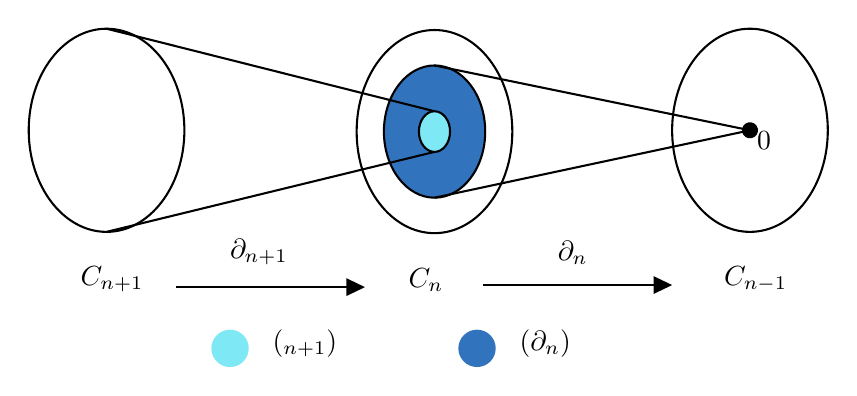
\begin{tikzpicture}[x=0.75pt,y=0.75pt,yscale=-1,xscale=1]
%uncomment if require: \path (0,300); %set diagram left start at 0, and has height of 300

%Shape: Ellipse [id:dp027523575399996947]
\draw  [fill={rgb, 255:red, 50; green, 115; blue, 190 }  ,fill opacity=1 ] (172.13,110.56) .. controls (172.13,92.97) and (183.06,78.71) .. (196.54,78.71) .. controls (210.02,78.71) and (220.94,92.97) .. (220.94,110.56) .. controls (220.94,128.15) and (210.02,142.41) .. (196.54,142.41) .. controls (183.06,142.41) and (172.13,128.15) .. (172.13,110.56) -- cycle ;
%Shape: Ellipse [id:dp6715234856450412]
\draw   (1,109.94) .. controls (1,82.91) and (17.79,61) .. (38.5,61) .. controls (59.21,61) and (76,82.91) .. (76,109.94) .. controls (76,136.97) and (59.21,158.88) .. (38.5,158.88) .. controls (17.79,158.88) and (1,136.97) .. (1,109.94) -- cycle ;
%Shape: Ellipse [id:dp5970693035579542]
\draw   (159,110.56) .. controls (159,83.53) and (175.79,61.62) .. (196.5,61.62) .. controls (217.21,61.62) and (234,83.53) .. (234,110.56) .. controls (234,137.59) and (217.21,159.5) .. (196.5,159.5) .. controls (175.79,159.5) and (159,137.59) .. (159,110.56) -- cycle ;
%Shape: Ellipse [id:dp677120237183229]
\draw   (311,109.94) .. controls (311,82.91) and (327.79,61) .. (348.5,61) .. controls (369.21,61) and (386,82.91) .. (386,109.94) .. controls (386,136.97) and (369.21,158.88) .. (348.5,158.88) .. controls (327.79,158.88) and (311,136.97) .. (311,109.94) -- cycle ;
%Straight Lines [id:da5084323464038256]
\draw    (38.5,61) -- (196.5,100.77) ;
%Straight Lines [id:da0593656829770326]
\draw    (38.5,158.88) -- (196.5,120.35) ;
%Shape: Ellipse [id:dp90627516544786]
\draw  [fill={rgb, 255:red, 126; green, 232; blue, 244 }  ,fill opacity=1 ] (189,110.56) .. controls (189,105.16) and (192.36,100.77) .. (196.5,100.77) .. controls (200.64,100.77) and (204,105.16) .. (204,110.56) .. controls (204,115.97) and (200.64,120.35) .. (196.5,120.35) .. controls (192.36,120.35) and (189,115.97) .. (189,110.56) -- cycle ;
%Straight Lines [id:da27148965742771414]
\draw    (196.54,78.71) -- (348.5,109.94) ;
%Straight Lines [id:da2680900125601313]
\draw    (196.54,142.41) -- (348.5,109.94) ;
\draw [shift={(348.5,109.94)}, rotate = 347.94] [color={rgb, 255:red, 0; green, 0; blue, 0 }  ][fill={rgb, 255:red, 0; green, 0; blue, 0 }  ][line width=0.75]      (0, 0) circle [x radius= 3.35, y radius= 3.35]   ;
%Straight Lines [id:da6647768815658852]
\draw    (72,185.5) -- (160,185.5) ;
\draw [shift={(163,185.5)}, rotate = 180] [fill={rgb, 255:red, 0; green, 0; blue, 0 }  ][line width=0.08]  [draw opacity=0] (8.93,-4.29) -- (0,0) -- (8.93,4.29) -- cycle    ;
%Straight Lines [id:da8110837686459536]
\draw    (220,184.5) -- (308,184.5) ;
\draw [shift={(311,184.5)}, rotate = 180] [fill={rgb, 255:red, 0; green, 0; blue, 0 }  ][line width=0.08]  [draw opacity=0] (8.93,-4.29) -- (0,0) -- (8.93,4.29) -- cycle    ;
%Shape: Circle [id:dp42521749904572537]
\draw  [draw opacity=0][fill={rgb, 255:red, 126; green, 232; blue, 244 }  ,fill opacity=1 ] (89,215) .. controls (89,210.03) and (93.03,206) .. (98,206) .. controls (102.97,206) and (107,210.03) .. (107,215) .. controls (107,219.97) and (102.97,224) .. (98,224) .. controls (93.03,224) and (89,219.97) .. (89,215) -- cycle ;
%Shape: Circle [id:dp32778703378474483]
\draw  [draw opacity=0][fill={rgb, 255:red, 50; green, 115; blue, 190 }  ,fill opacity=1 ] (208,215) .. controls (208,210.03) and (212.03,206) .. (217,206) .. controls (221.97,206) and (226,210.03) .. (226,215) .. controls (226,219.97) and (221.97,224) .. (217,224) .. controls (212.03,224) and (208,219.97) .. (208,215) -- cycle ;

% Text Node
\draw (24.5,173.9) node [anchor=north west][inner sep=0.75pt]    {$C_{n+1}$};
% Text Node
\draw (182.5,174.9) node [anchor=north west][inner sep=0.75pt]    {$C_{n}$};
% Text Node
\draw (334.5,173.9) node [anchor=north west][inner sep=0.75pt]    {$C_{n-1}$};
% Text Node
\draw (350.5,109.18) node [anchor=north west][inner sep=0.75pt]    {$0$};
% Text Node
\draw (96.5,160.9) node [anchor=north west][inner sep=0.75pt]    {$\partial _{n+1}$};
% Text Node
\draw (254.5,161.9) node [anchor=north west][inner sep=0.75pt]    {$\partial _{n}$};
% Text Node
\draw (117,204.4) node [anchor=north west][inner sep=0.75pt]    {$\Ima( \boundary_{n+1})$};
% Text Node
\draw (236,204.4) node [anchor=north west][inner sep=0.75pt]    {$\Ker( \partial_{n})$};


\end{tikzpicture}
